\chapter{Introducción}


Hace aproximadamente 400 años Johannes Keppler usó  mediciones precisas de cuerpos celestes realizadas por Tycho Brahe para derivar reglas geométricas que relacionan sus órbitas con sus períodos. Luego, a partir de las leyes propuestas por Newton, incluyendo la ley de gravitación universal, y conociendo sus condiciones iniciales así como las interacciones con otros planetas dentro del sistema, fue posible predecir sus trayectorias. Además de incluir las leyes de Kepler, este formalismo introdujo un nivel de detalle más profundo que permitió encontrar incongruencias entre las predicciones de las trayectorias con observaciones y así inferir interacciones faltantes, como fue el caso del descubrimiento de Neptuno a partir de la discrepancia entre la órbita predicha y la observada de Urano.

En biología los comportamientos dependen de una intrincada red de proteínas y genes que interactúan entre sí para responder acorde a las necesidades del organismo y el entorno en el que se hayan inmersos. La biología de sistemas propone una visión holística en donde se analizan las complejas interacciones entre especies en búsqueda de comportamientos emergentes, en contraposición a una visión más Mendeliana donde se relaciona ``un gen - un fenotipo'' \citep{Han2008}. En dichas redes, cada nodo representa alguna biomolécula (proteína, gen, metabolito, etc), mientras que sus interacciones están dadas por relaciones funcionales (transcripción, traducción, modificación genética, modificación postraduccional, reacción metabólica, entre otras). Plasmar estas redes en modelos resulta útil para transferir de forma concisa conocimientos previos e hipótesis de un sistema, así como para predecir comportamientos que tienen que ser verificados experimentalmente \citep{Aldridge2006}. A medida que nuestro conocimiento sobre éste aumenta, los modelos pueden evolucionar con la nueva información adquirida y así hacer predicciones más certeras \citep{Vayttaden2004}. 


%%%%%%%%%%%%%%%%%%%%%%%%%%%%%%%%%%%%%%%%
\section{Cómo estudiar redes biológicas}
\label{sec:intro:EstudiarRedes}


La identificación y descripción de los elementos que componen un sistema, así como sus interacciones, es el primer paso de la difícil tarea de dilucidar el funcionamiento de la maquinaria celular \citep{Grecco2008}. Comprender el funcionamiento de las partes a partir del producto final se engloba dentro de los denominados ``problemas inversos'', en particular, ingeniería inversa. Es de conocimiento general que hay problemas que son fáciles de resolver en un sentido, pero muy complicados para comprender en el sentido inverso. Sin ir más lejos, no es complicado calcular derivadas, pero sabemos que no siempre podemos resolver integrales fácilmente \citep{Milotti2013}.

Las redes biológicas usualmente comienzan siendo descriptas como simples diagramas de bloques donde solo se muestran influencias entre especies, sin detallar las características de dicha influencia. \cite{Ahn1990} presentaron un análisis donde muestran la vía de proteínas quinasas activadas por mitógenos (MAPK) pero no queda claro si éstas se activan en forma simultánea o secuencial. A continuación, entre 1991 y 1993, se publicaron una serie de trabajos en los que se describían interacciones mostrando una activación secuencial mediante fosforilaciones (adición de grupos fosfato) mediadas por quinasas que fosforilan otras quinasas \citep{Ahn1991, Itoh1993}. Estos modelos sentaron las bases sobre las que se fueron construyendo los sucesivos modelos a medida que se dilucidaban más detalles (ver \cref{fig:evolucion_modelos} cuadros rojos).

\begin{figure}
    \centering
    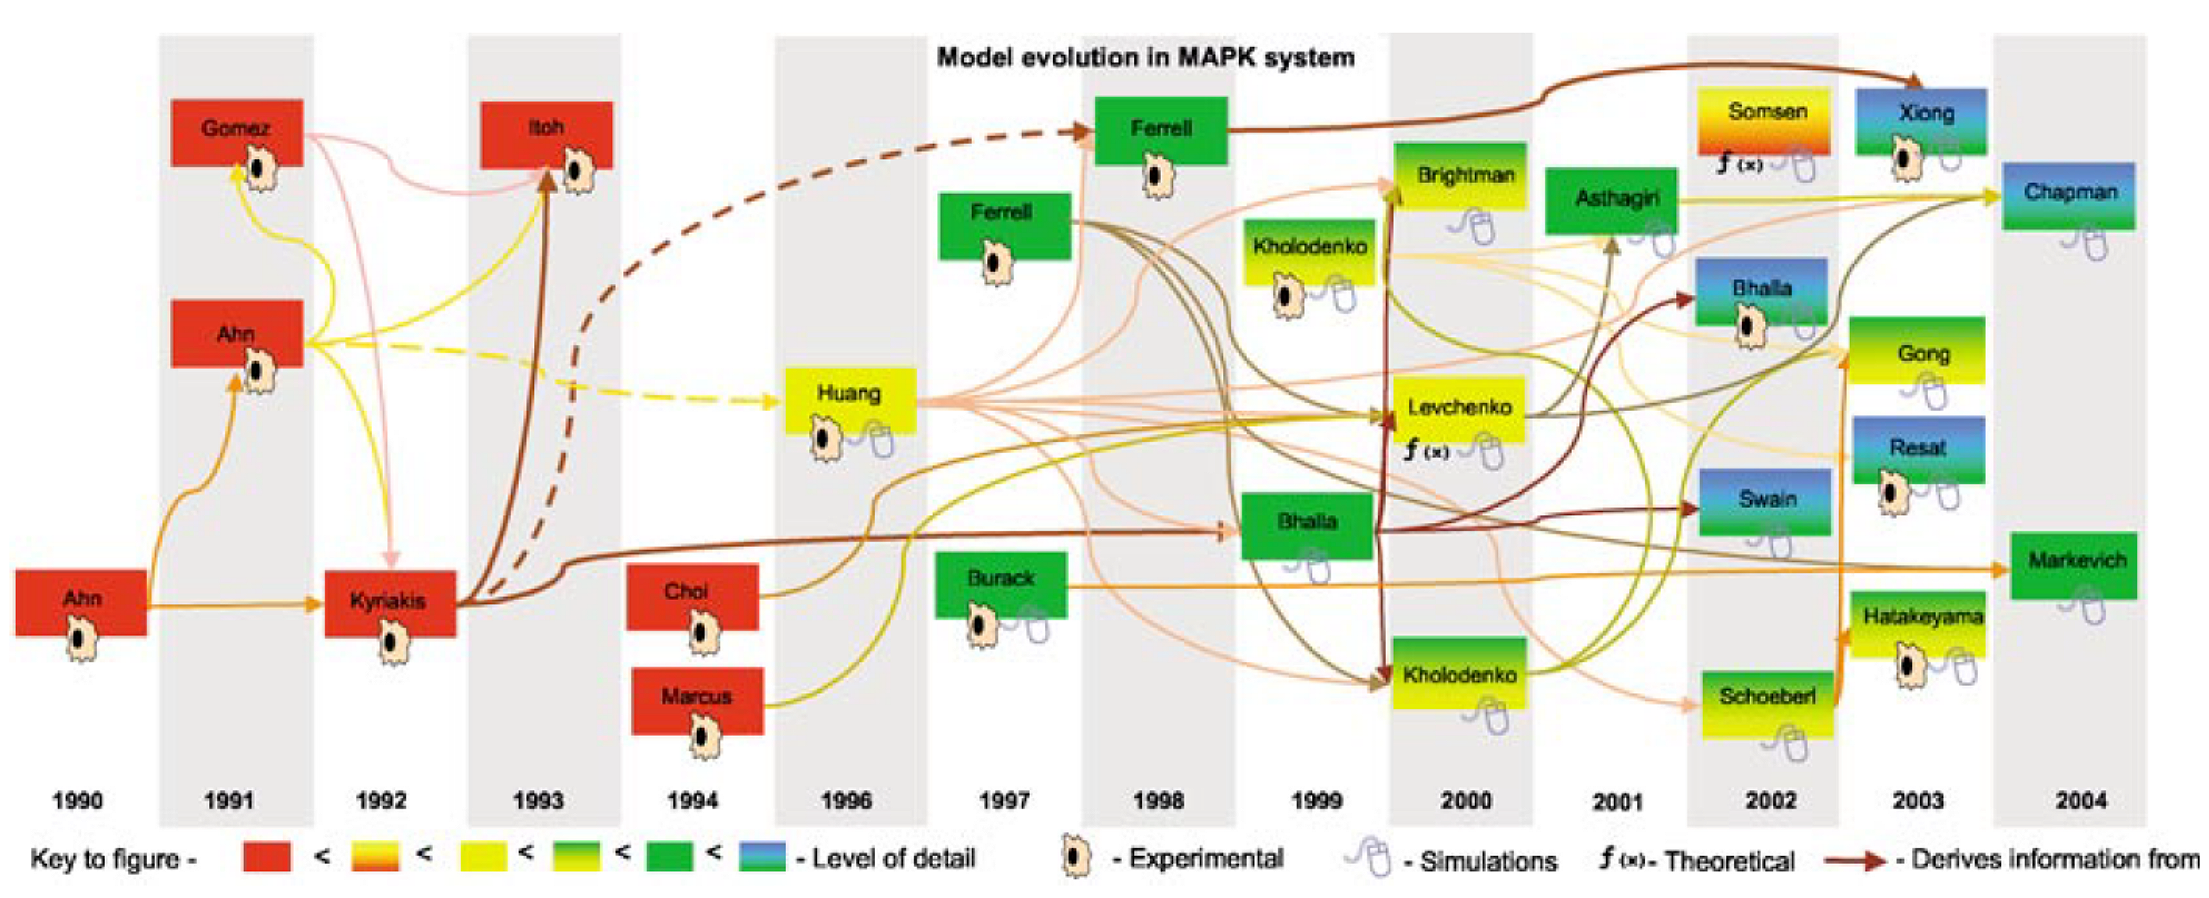
\includegraphics[width=0.8\textwidth]{img/cap_1/model_evolution.png}
    \caption{\footnotesize{Evolución del modelado de la cascada de MAPK. De izquierda a derecha el año en que se introdujo el modelo, y cada modelo se haya en una caja cuyo color representa su nivel de detalle. Éste nivel puede ir desde una mera descripción de las partes y las influencias entre ellas (como los casos rojos), a modelos simples con parámetros de prueba que demuestran comportamientos emergentes (cuadros amarillos), y hasta modelos en donde la dinámica de las interacciones esta cuantificada y existe un correlato experimental de la mecánica del modelo (cuadros azules y verdes). Debajo de cada modelo se detalla que tipo de modelado se usó y las flechas conectan fuentes de información utilizadas. Imagen tomada de \cite{Vayttaden2004}.}}
    \label{fig:evolucion_modelos}
\end{figure}

Al obtener más detalles sobre el tipo de interacciones entre especies, se llega a modelos de sistemas en los que es posible identificar motivos repetidos \citep{Tyson2003}. Aunque algunas redes pequeñas fueron delineadas con un elevado nivel de detalle, se estima que por ejemplo existen como mínimo unas 150000 interacciones proteicas en humanos, y para estudiarlas es necesario implementar técnicas de alto rendimiento \citep{Han2008}. Entre estas técnicas se encuentran inmunoprecipitación de cromatina seguido de identificación por microarray (ChIP-chip) o secuenciación (ChIP-seq) para interacciones entre factores de transcripción y genes, o purificación de co-afinidad seguido de identificación por espectroscopia de masa para interacciones entre proteínas. Por ejemplo, \cite{Soderberg2008} desarrollaron un protocolo para realizar ensayos de ligadura de proximidad \textit{in situ} y así determinar en qué compartimientos ocurren dichas interacciones. \cite{Berggard2007} confeccionaron un resumen de distintas técnicas para marcar qué proteínas interactúan entre sí. En el caso de \cite{Kang2020}, en donde utilizan inmunoprecipitación de cromatina para identificar interacciones entre factores de transcripción y ADN. Cuando la cantidad de especies e interacciones es elevada, es común hallar implementaciones de redes bayesianas donde se perturban las concentraciones de varias especies y se analizan los efectos sobre otras, como muestran \cite{Xu2010} y \cite{Sachs2005}. \cite{Mootha2003} logran asociar el origen de la deficiencia de citocromo C oxidasa a un gen a través de integración de datos de co-expresión genética, proteómica y un mapa físico de loci candidatos a enfermedad. Estos métodos permiten reconstruir las redes biológicas cuya dinámica posteriormente se interroga para generar modelos bioquímicos.

Los modelos de bioquímica celular en general se basan en la ley de acción de masas para describir las reacciones químicas. Estos pueden estar basados en diversos formalismos matemáticos, desde lógica booleana hasta ecuaciones diferenciales ordinarias. A través de la ley de acción de masas, las variaciones en las concentraciones de cada especie se pueden predecir cuantitativamente a partir de las constantes de reacción que describen sus interacciones, incluso entre distintas escalas \citep{Krakauer2011}. Agregar dichas constantes permite desarrollar modelos numéricos que pueden ser matemáticamente integrados. En el trabajo de \cite{Huang1996} se utilizan las descripciones previas de la cascada de MAPK para generar un modelo matemático simple con parámetros de prueba y demostrar un comportamiento emergente de la red en el que ésta responde fuertemente a la señal de estímulo una vez superada cierta concentración crítica, denominado ultrasensibilidad (ver \cref{fig:evolucion_modelos} cuadros amarillos).

Es común hallar en la literatura que a medida que se realizan nuevos experimentos se modifican o confeccionan modelos que describan dichos resultados, sin verificar si se mantienen predicciones previas. Idealmente se deberían agregar datos de experimentos previos y los nuevos experimentos servirían para, iterativamente, evaluar y refinar el modelo. Además, integrar modelos que contienen especies en común representa un avance en el desarrollo de modelos más completos, e incluso, modelos de célula completa como sugieren \cite{Karr2015}. Sin embargo, no siempre es posible agregar datos entre sí ya que no hay herramientas desarrolladas para tal propósito. La falta de acceso a algunos modelos, su incompatibilidad entre ellos, errores de formato o insuficiente información sobre como implementarlos son algunos de los inconvenientes usuales mencionados por \cite{Szigeti2018} a la hora de transferir modelos dentro de la comunidad.

Con el objetivo de combatir las dificultades en la transferencia de modelos, año a año se desarrollan nuevas herramientas que permiten publicar y compartir modelos, facilitando así su evaluación y refinamiento. En el trabajo de \cite{Hucka2003}, se presenta un lenguaje basado en XML, \ening{Systems Biology Markup Language} (SBML), que es utilizado para representar e intercambiar modelos de redes bioquímicas. Modelos descriptos en dicho lenguaje pueden ser subidos a distintos repositorios públicos, como el presentado por \cite{Malik-Sheriff2018}, denominado \ening{BioModels}. Bionetgen (BNGL), otro lenguaje de modelado, se basa en definir reglas de interacción entre especies, permitiendo definir en pocas líneas cómo ensamblar un polímero a partir de monómeros \citep{Harris2016}.

Asimismo, los modelos de ecuaciones diferenciales ordinarias suelen basarse en la ley de acción de masas donde las velocidades de reacción son proporcionales a las concentraciones de los reactivos \citep{Sorger2011}. Esta cinética de acción de masas es una aproximación continua a una descripción más fundamental, discreta y estocástica, que es la ecuación maestra. Como hipótesis se asume que los reactivos se encuentran bien mezclados y que el sistema se halla en equilibrio termodinámico, pero no necesariamente en equilibrio químico \citep{Chen2010}. \cite{Bhalla2002} analiza mediante estos métodos \textit{in silico} cómo la cascada de señalización de MAPK regula la sensibilidad al ligando por medio de una retroalimentación positiva entre la fosfatasa de MAPK y la proteína quinasa C (PKC) (ver \cref{fig:evolucion_modelos} cuadros azules). La dimensión espacial tiene diversos efectos sobre el sistema que pueden ser agregados utilizando ecuaciones en derivadas parciales. Este tipo de ecuaciones representan sistemas bioquímicos en tiempo y espacio continuos y modelan fenómenos de difusión, gradientes de concentración y transporte \citep{Sorger2011}. Los mismos fueron aplicados por \cite{Rehm2009} para modelar las ondas espaciales de permeabilización de membrana mitocondrial externa, encontrando y explicando por qué células hijas inician la apoptosis de forma sincrónica.

Por otro lado, el enfoque estocástico trata la evolución temporal de las variables dinámicas del sistema de forma discreta y análoga a las caminatas al azar. Considerando el carácter aleatorio que tienen las colisiones moleculares en las reacciones químicas, se utiliza una ecuación que describe la probabilidad de variación de la variable dinámica. A continuación se generan números aleatorios siguiendo las probabilidades calculadas o utilizando el método de Monte Carlo, simulando así la variable deseada \citep{Gillespie1977}. Como muestra \cite{Gillespie1977}, estos métodos pueden reproducir los resultados que provee una ecuación maestra para concentraciones homogéneas, además de proveer información valiosa sobre las fluctuaciones de la variable analizada. El modelo teórico de \cite{Friedman2006} logra reconciliar la variación temporal con las mediciones realizadas en una población celular basándose en el mecanismo de producción de proteínas subyacente. Por último, cabe destacar que las fluctuaciones de las reacciones son del orden de $1/\sqrt{N}$, siendo $N$ la cantidad de moléculas disponibles para reaccionar. Luego, si $N>10^2$ podemos usar un modelo determinista continuo despreciando estas fluctuaciones \citep{Chen2010}.

% A través de la ley de acción de masas, las variaciones en las concentraciones de cada especie se pueden predecir cuantitativamente a partir de las constantes de reacción que describen sus interacciones y entre las distintas escalas \citep{Krakauer2011}. Al agregar dichas constantes podemos desarrollar modelos numéricos que pueden ser matemáticamente integrados. Esta evolución de modelos se encuentra ejemplificada en el trabajo de \cite{Vayttaden2004} para el caso de la vía de proteínas quinasas activadas por mitógenos (MAPK, ver \cref{fig:evolucion_modelos}). \cite{Bhalla2002} analizan mediante metodos \textit{in silico} como la cascada de señalizacón de MAPk regulan la sensibilidad al ligando por medio de una retroalimentación positiva entre la fosfatas de MAPK y la proteín quinasa C (PKC).

Analicemos a forma de ejemplo el operón lactosa de \textit{escherichia coli}: la alolactosa puede unirse al represor de lactosa quien, a su vez, interactúa fuertemente con el ADN evitando que ARN polimerasas puedan acceder para transcribir ciertos genes. Cuando se alcanza cierta concentración crítica de alolactosa, ésta se une al represor haciendo que se desligue del ADN y permitiendo la síntesis del operón que codifica, entre otras proteínas, para una permeasa que permite el ingreso a la célula de más alolactosa. Cabe destacar que éste es un sistema autocatalítico ya que, una vez que se sintetizó permeasa, más alolactosa entra a la célula estimulando la síntesis de más permeasa \citep{Laurent1999}. Este tipo de red de interacciones se repite frecuentemente en sistemas biológicos ya que genera un comportamiento de tipo interruptor en respuesta a alguna variable (ver \cref{fig:switch}).

\begin{figure}
    \centering
    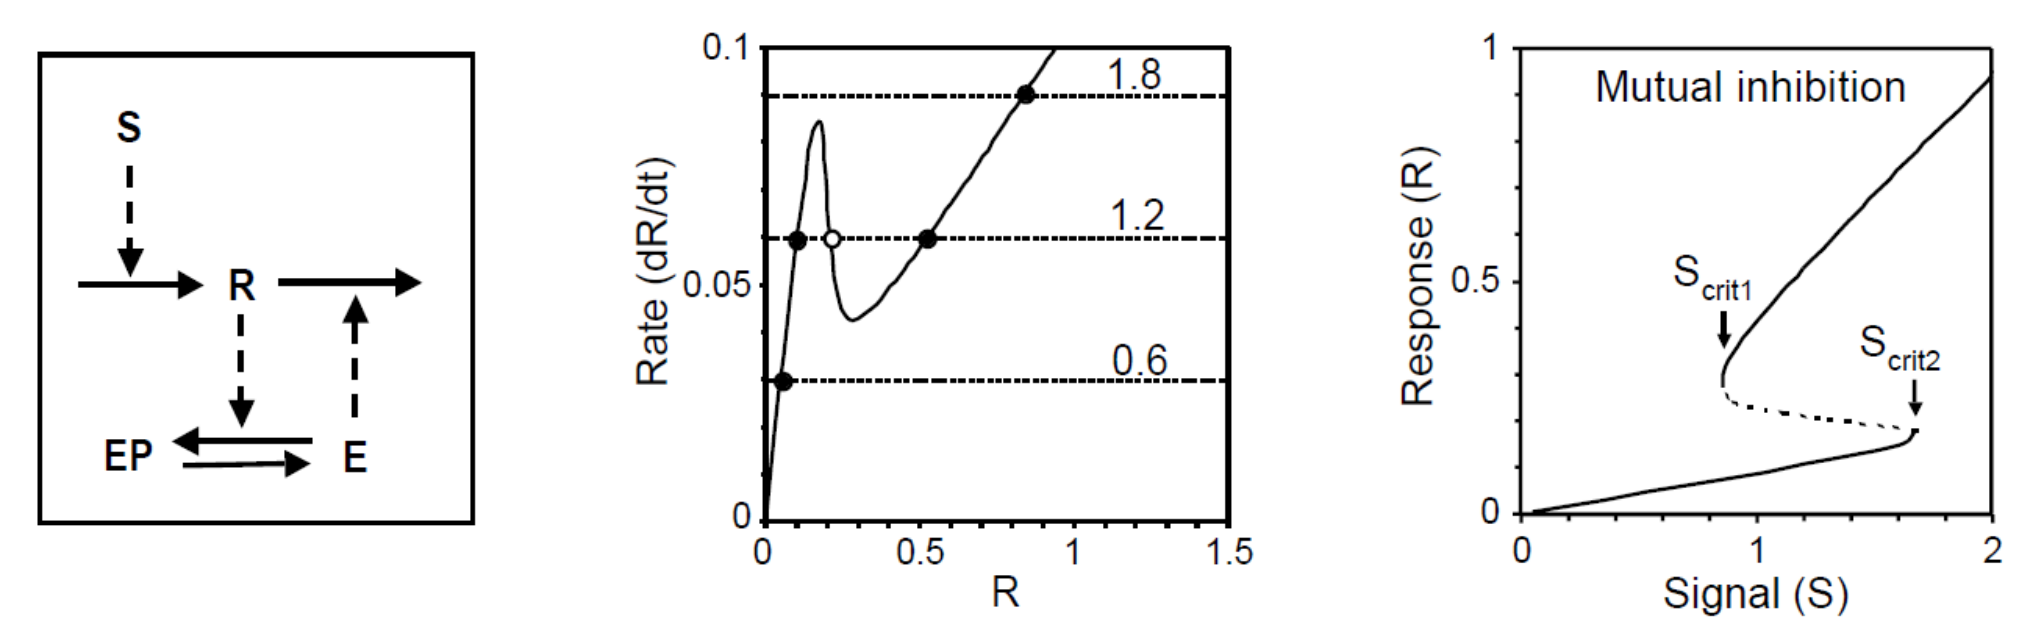
\includegraphics[width=0.8\textwidth]{img/cap_1/switch_example.png}
    \caption{\footnotesize{A la izquierda se puede ver un diagrama de las interacciones entre las especies en donde S representa alguna señal, R la respuesta del sistema y E es una especia que interactúa con R. En el ejemplo del operón de lactosa: S representa la alolactosa, R la permeasa y E el inhibidor. En el medio se grafica el cambio de concentración de la respuesta respecto al tiempo en función de R. A la derecha se muestra el diagrama de fases de la respuesta en función de la señal. Imagen tomada de \cite{Tyson2003}.}}
    \label{fig:switch}
\end{figure}

Debemos destacar en el modelo presentado anteriormente que las escalas temporales de las reacciones pueden diferir en varios ordenes de magnitud. En particular, el cambio conformacional del represor al unirse a alolactosa puede ser del orden de segundos mientras que el tiempo que tarda en sintetizarse o degradarse la permeasa está en el orden de horas. Además, las especies pueden representar distintas variantes de proteínas o complejos. En señalización intracelular suele ocurrir que el cambio que se propaga a través de la red son modificaciones postraduccionales, como fosforilaciones en sitios específicos de cada proteína y ocurren en el orden de minutos. Dependiendo el nivel de detalle del modelo, es posible tomar aproximaciones sobre distintas escalas temporales o incluso agrupar especies o reacciones en una sola.

Sistemas como el operón lactosa se hallan inmersos en una red más amplia y compleja dentro del organismo. Adicionalmente, en organismos más evolucionados, éstas redes suelen ser más grandes. Al incluir más especies con sus respectivas interacciones en un modelo, éste aumenta en complejidad. Entre las complicaciones del diseño de modelos se encuentran la dificultad de poder interpretarlos intuitivamente cuando se tienen muchos motivos interconectados y la extensión del espacio de parámetros \citep{Tyson2020}.

Separar el modelo en distintos módulos, cuando es posible, facilita tanto la interpretación de éste como la determinación de qué especies observar o perturbar  experimentalmente. Como muestran \cite{Harrington2008}, para estudiar la cascada apoptótica combinan las vías extrínseca e intrínseca mediante la implementación de módulos funcionales y subredes ya descriptas en la bibliografía para modelarla y además determinar su dinámica. Por otro lado, el análisis de respuesta modular (\ening{Modular Response Analysis}, MRA) consiste en separar la red en módulos de forma tal que solo hayan algunas especies que sirvan de mediadoras entre módulos. El desarrollo de dicho método y su aplicación a la cascada de MAPK y la regulación de asimilación de amonio en \textit{escherichia coli} fue introducido por \cite{Bruggeman2002}. En el trabajo de \cite{Santos2007}, se utiliza MRA para distinguir las diferencias en respuesta de la cascada MAPK ante estímulos distintos (ver \cref{fig:mra_ejemplo}). Aplicándolo descubren cómo al utilizar factor de crecimiento nervioso (NGF) aparece un lazo de retroalimentación positivo en lugar de uno negativo, como cuando se utiliza factor de crecimiento epidérmico (EGF). Estos tipos de análisis permiten reconstruir los comportamientos emergentes de la interacción entre distintos módulos de una red extensa.

\begin{figure}
    \centering
    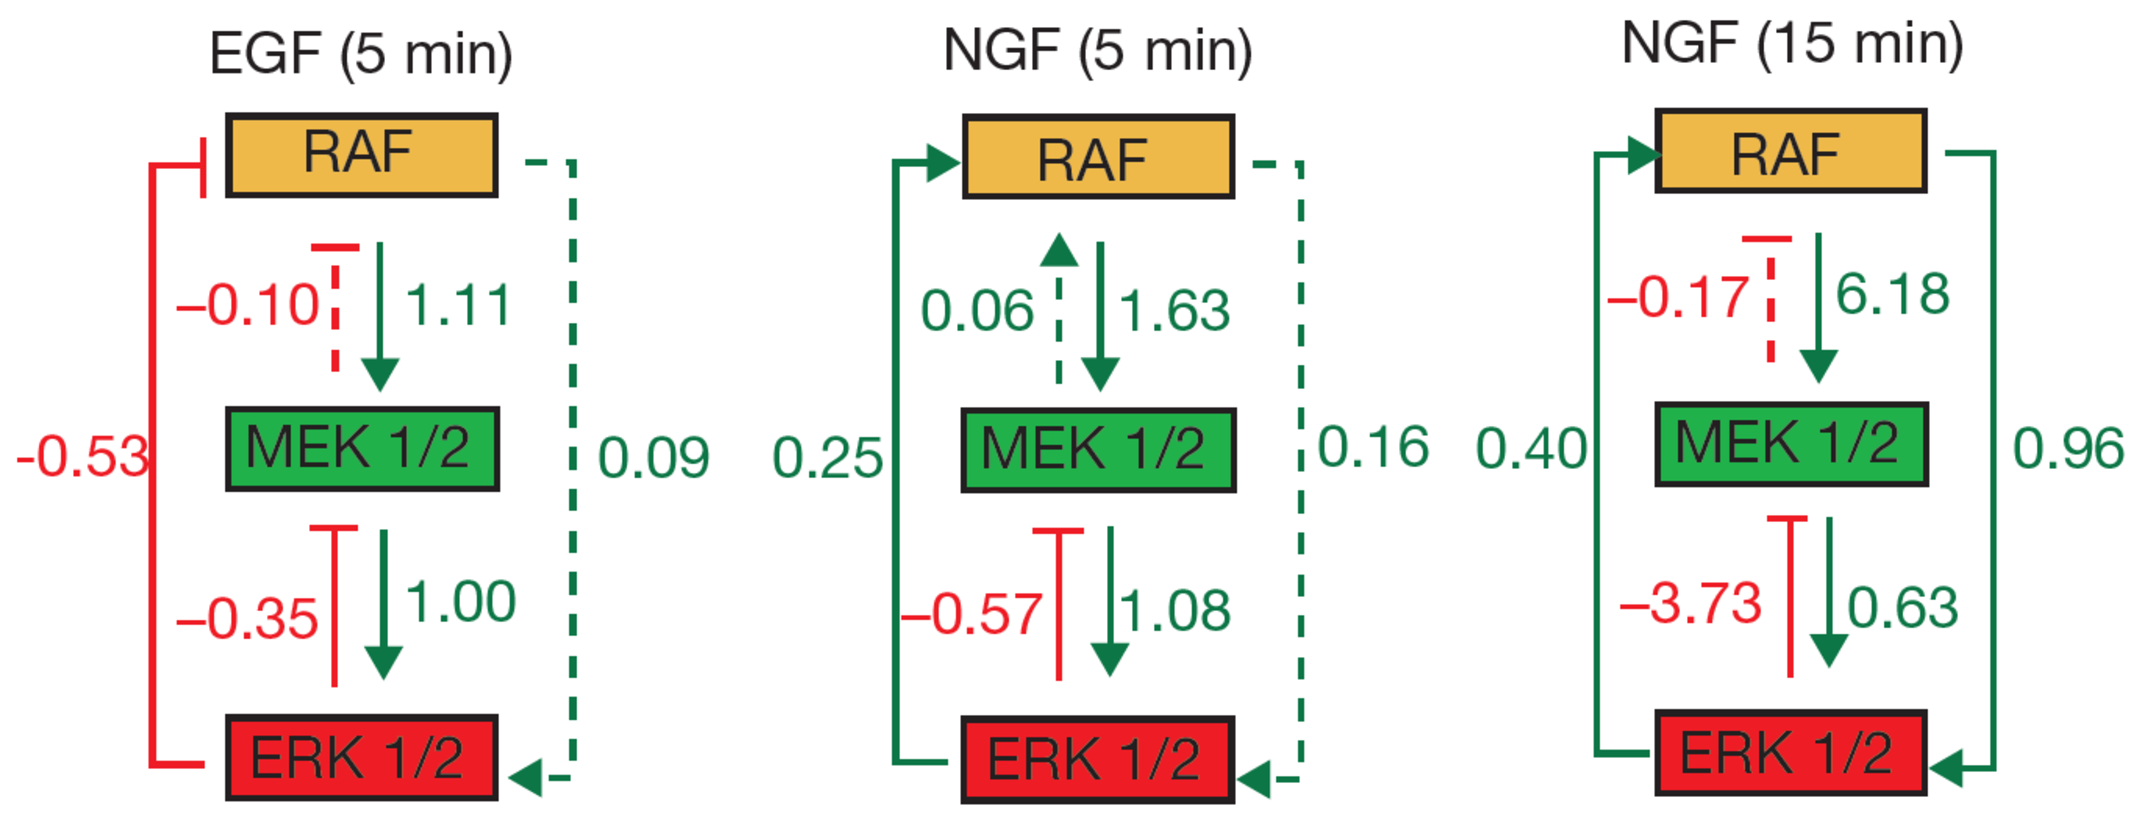
\includegraphics[width=0.6\textwidth]{img/cap_1/mra_example.pdf}
    \caption{\footnotesize{Resultados del análisis de MRA aplicado al estudio de la cascada de MAPK al utilizar dos estímulos distintos y a tiempos distintos. Imagen tomada de \cite{Santos2007}.}}
    \label{fig:mra_ejemplo}
\end{figure}

En todo tipo de modelado existe un equilibrio que debe encontrarse entre el nivel de detalle buscado y la complejidad inherente de su análisis. Modelos que consideran gran cantidad de variables e interacciones pueden ser muy detallistas y precisos, pero son más difíciles de ajustar experimentalmente, considerando la cantidad de constantes de reacción y condiciones iniciales que deben determinarse \citep{Sorger2011}. Cada interacción incluida en un modelo agrega los parámetros correspondientes a sus constantes cinéticas, mientras que cada especie va a traer aparejada su concentración inicial. Aunque algunos de estos parámetros refieren a especies intermedias cuya concentración inicial es cero, otros parámetros pueden ser muy variables en una población celular, como se aprecia en el trabajo de \cite{Spencer2009}, donde las concentraciones iniciales del modelo son tomadas aleatoriamente de una distribución lognormal. Por otro lado, en algunos casos hay más de una combinación de parámetros que reproducen soluciones indistinguibles desde un punto de vista experimental. Aunque se invierte mucho esfuerzo en determinar los parámetros para los modelos, algunos trabajos destacan la importancia de identificar adecuadamente la topología de la red en lugar de la mejor combinación de parámetros. \cite{Frohlich2018} desarrolla un método para acelerar considerablemente las simulaciones de sus modelos, y así realizar un análisis más exhaustivo de cómo la variación en los parámetros afecta la incertidumbre de ciertos observables. Por otro lado, en el trabajo de \cite{Santolini2018} se afirma que un 65\%-80\% de la precisión de los modelos depende de encontrar adecuadamente la topografía de la red, y lo remanente a determinar correctamente los parámetros. A modo de ejemplo, \cite{Kraeutler2010} estudian la señalización $\beta$-adrenérgica de los cardiocitos modelándola mediante ecuaciones de Hill para las interacciones y muestran que pueden recuperar comportamientos clave sin necesidad de ajustar todos los parámetros.


%%%%%%%%%%%%%%%%%%%%%%%%%%%%%%%%%%%%%%%%
\section{Cómo interrogar la dinámica de redes biológicas}


Para interrogar redes biológicas resulta importante ser capaz de reportar la dinámica de actividad de distintos nodos de la red simultáneamente y a nivel de célula única debido a su inherente variabilidad. Durante los últimos tiempos, hubo una explosión en el desarrollo de biosensores genéticamente codificados que permitió cuantificar la actividad de diversas enzimas como proteína G acoplada a receptor (GPCR, ver \cref{fig:pthr}), quinasa regulada por señalización extracelular (ERK), quinasa c-Jun N-terminal (JNK), entre muchas otras, así como la presencia de moléculas pequeñas \citep{Greenwald2018}.

\begin{figure}
    \centering
    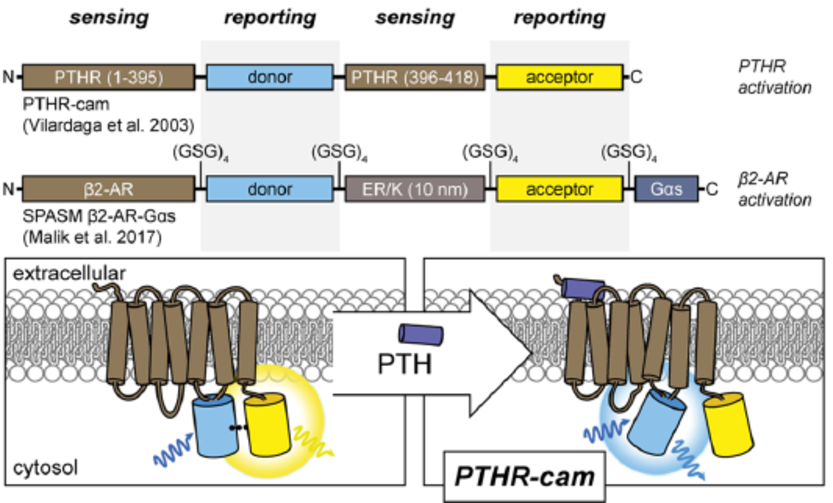
\includegraphics[width=0.65\textwidth]{img/cap_1/pthr.pdf}
    \caption{\footnotesize{Esquema de un sensor de un tipo de receptor asociado a proteína G llamado PTHR. Éste consiste en el receptor modificado para incluir a CFP como donante y YFP como aceptor. En su configuración basal, los fluoróforos se encuentran suficientemente cerca como para transferir energía por FRET de CFP a YFP, sin embargo, el cambio conformacional producido por la unión del ligando, PTH, aleja los fluoróforos entre sí, interrumpiendo dicha transferencia. Analizar el ratio de intensidad de emisión entre los canales cian y amarillo permitirá determinar el estado de la población de receptores. Imagen tomada de \cite{Greenwald2018}.}}
    \label{fig:pthr}
\end{figure}

El mecanismo de funcionamiento de estos reporteros consiste en diseñarlos de forma tal que sus propiedades espectroscópicas sean sensibles al entorno \citep{Bastiaens1999}. Mientras algunos de estos sensores no emiten fluorescencia en uno de estos estados, otros hacen uso de dos moléculas fluorescentes y la capacidad de intercambiar energía entre ellas a través de un proceso denominado Transferencia de Energía de Resonancia de Förster (FRET). Dicho fenómeno consiste en la transferencia de energía entre un fluoróforo y otro de manera no radiativa como resultado de un acoplamiento dipolo-dipolo. Para que esto ocurra, se deben dar varias condiciones: que la distancia entre ambos sea del orden de 5~nm, sus orientaciones lo permitan y que el espectro de emisión del donante se superponga con el de excitación del aceptor. Cabe recalcar que los biosensores basados en FRET se pueden clasificar en heteroFRET, si las especies de fluoróforos utilizados son distintos, u homoFRET, cuando son idénticos.

Los biosensores basados en heteroFRET son más ubicuos y, para estimar la eficiencia de FRET, se procede a excitar al dador y luego cuantificar la intensidad de la emisión del dador y aceptor en sus respectivos canales. \cite{Miyawaki1997} presentan en su trabajo un sensor basado en CFP y YFP conectados por calmodulina y un péptido M13 que se unen de forma reversible al ion de calcio (ver \cref{fig:bios}A). Dicho biosensor fue utilizado para estimar las concentraciones de calcio en distintos compartimientos celulares. Por otro lado, \cite{Grashoff2010} desarrollaron un biosensor compuesto por los fluoróforos mTFP1 y Venus, unidos por un segmento elástico, que fue utilizado para medir fuerzas entre proteínas. Una vez calibrados, este tipo de sensores permiten transducir eficiencia de FRET en tensión sensada y así estudiar la evolución de las fuerzas entre proteínas en adhesiones focales (ver \cref{fig:bios}B). La posibilidad de implementar este tipo de biosensores en células y organismos vivos permite obtener información sobre la temporalidad y espacialidad de distintas redes biológicas.

\begin{figure}[htb]
    \centering
    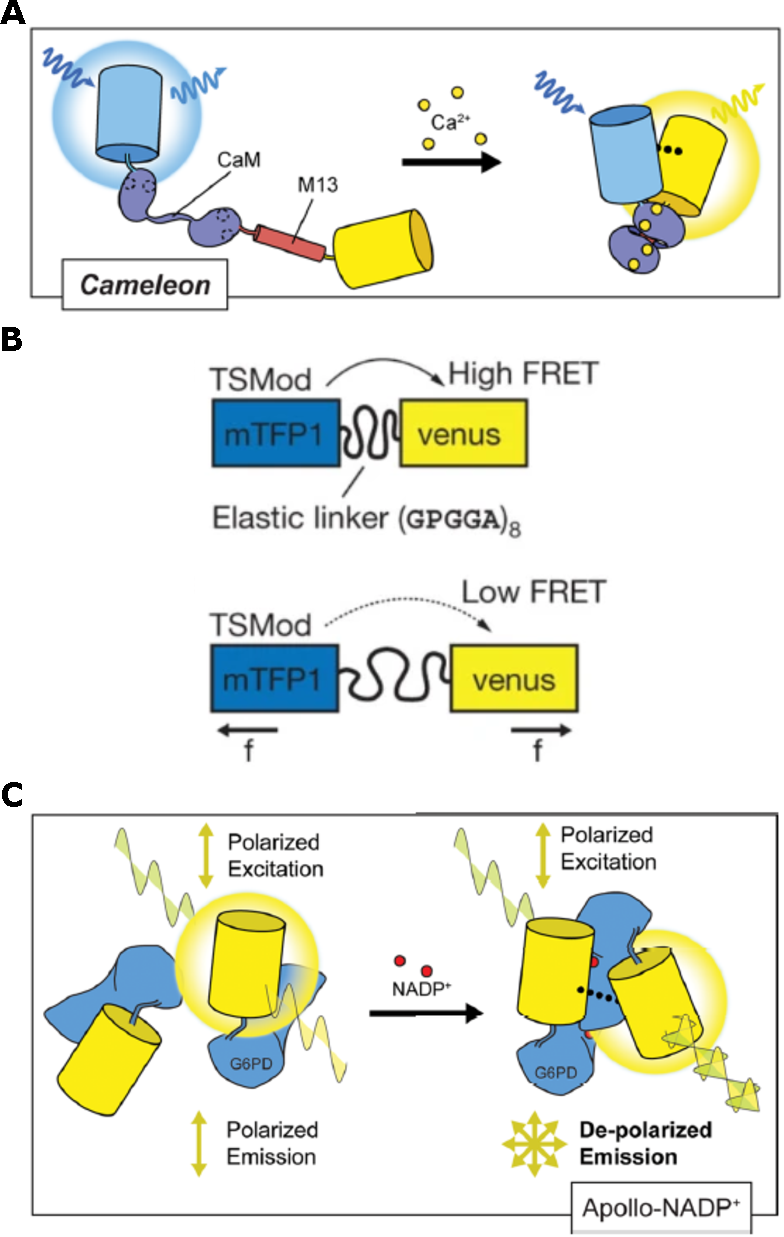
\includegraphics[width=0.5\textwidth]{img/cap_1/biosensors.pdf}
    \caption{\footnotesize{\textbf{A.} Esquema de un biosensor de calcio basado en heteroFRET y compuesto por CFP y YFP, unidos por calmodulina y un péptido M13. Imagen tomada de \cite{Greenwald2018}. \textbf{B.} Esquema de un sensor de fuerzas moleculares compuesto por mTFP1 y Venus, unidos por una secuencia elástica. Imagen tomada de \cite{Grashoff2010}. \textbf{C.} Esquema de un biosensor basado en homoFRET y capaz de sensar la presencia de NADPH en las células. Imagen tomada de \cite{Greenwald2018}.}}
    \label{fig:bios}
\end{figure}

En el caso de los biosensores basados en homoFRET, en lugar de utilizar distintos canales de emisión para analizar la eficiencia de FRET, se utiliza microscopía de anisotropía de polarización. Considerando que el eje de excitación de las proteínas fluorescentes es casi paralelo al de emisión y dado que el tiempo de vida de fluorescencia en citoplasma ($\sim2.6$~ns) es considerablemente menor que el tiempo de correlación rotacional ($\sim36$~ns), ésta microscopía consiste en excitar la muestra con luz polarizada para realizar una fotoselección y luego analizar la anisotropía de fluorescencia, estudiando la emisión en la polarización paralela y perpendicular a la excitación  \citep{Swaminathan1997}. Si los fluoróforos fotoseleccionados son monoméricos tendrán una emisión anisótropa, mientras que si se encuentran en estado dimérico la emisión será más isótropa ya que por FRET parte de la emisión será en el eje del fluoróforo aceptor que no se encuentra necesariamente paralelo al donante. \cite{Cameron2016} desarrollaron Apollo, un biosensor basado en homoFRET para sensar el estado redox de la célula y muestran como NADPH se depleta en células $\beta$ previo a la acumulación de peróxido de hidrógeno (ver \cref{fig:bios}C). Una gran ventaja de utilizar este tipo de biosensores es que tienen un ancho espectral mucho menor y no es necesario utilizar dos canales distintos para observar el dador y el emisor, permitiendo multiplexar señales de más biosensores, como muestran \cite{Warren2015} al combinar un sensor de heteroFRET para calcio y uno de homoFRET para cúmulos de fosfatidilinostol.

% Estudiar la orientación del fluoróforo unido a la cabeza de myosina (S$_1$) permitió identificar su disposición y orientación al unirse a F-actina. En el trabajo de \cite{Andreev1993}, se concluyó que S$_1$ podía unirse de dos formas distintas según se halle en exceso o déficit en relación a la cantidad de F-actina. Conociendo el efecto que tiene la viscosidad del medio sobre el tiempo de correlación de rotación del fluoróforo, la anisotropía de fluorescencia puede ser utilizada para obtener información sobre parámetros reológicos del citosol, como se muestra en el trabajo de \cite{Swaminathan1997}. Por otro lado, dado que la unión del fluoróforo a otra molécula produce un cambio en la anisotropía, se la puede utilizar para reportar la proporción de fluoróforos ligados entre el total de fluoróforos. \cite{Dubach2014} utilizan esta técnica \textit{in vivo} para observar la dinámica de interacción entre la droga y su blanco (Olaparib) en tiempo real, mostrando su utilidad para descifrar la dinámica intracelular.

Tradicionalmente, los estudios de las interacciones involucradas en señalización dependían de análisis \textit{in vitro} como Western Blot o ensayos enzimáticos. En el caso de los Western Blots, se somete a una población celular a un tratamiento particular y luego se procede a lisar y recuperar el contenido intracelular de la población, del compartimiento de interés, y cuantificarlo. Éstos métodos continúan siendo importantes para determinar las interacciones entre especies, pero las ventajas introducidas por los biosensores fluorescentes genéticamente codificados los hace cruciales para estudiar la dinámica temporal de las señales. \cite{Ryu2015} retoman el estudio de como células PC12 responden de forma distinta ante EGF y NGF, y mediante la implementación de EKAR, un biosensor basado en heteroFRET que cambia su conformación al ser fosforilado en una subunidad de ERK, encuentran que el tipo de respuesta se encuentra codificado en la frecuencia de la señalización (ver \cref{fig:dinamica_temporal}A). Es fácil ver que si el sistema en estudio presenta oscilaciones, cualquier técnica que promedie en una población celular o carezca de información temporal, no será útil para estudiarlas. Con esto en mente, \cite{Barbosa1998} utilizan Fura-2 para relacionar las oscilaciones de Calcio intracelular en células $\beta$ generadas por niveles elevados de glucosa extracelular y la subsecuente liberación pulsada de insulina (ver \cref{fig:dinamica_temporal}B). \cite{Fosbrink2010} desarrollan el biosensor JNKAR1 para estudiar la como la vía JNK integra señales de supervivencia o muerte celular. Éste biosensor esta basado en heteroFRET y aumenta 15 a 30\% el ratio de emisión de amarillo a cyan una vez fosforilado. Por medio de dicho biosensor sientan las bases de la dinámica de la cascada JNK demostrando la rapidez con que se propaga la señal dentro de la célula, su carácter biestable, ultrasensible y bimodal ante estímulos ribotóxicos como anisomicina (ver \cref{fig:dinamica_temporal}C).

\begin{figure}
    \centering
    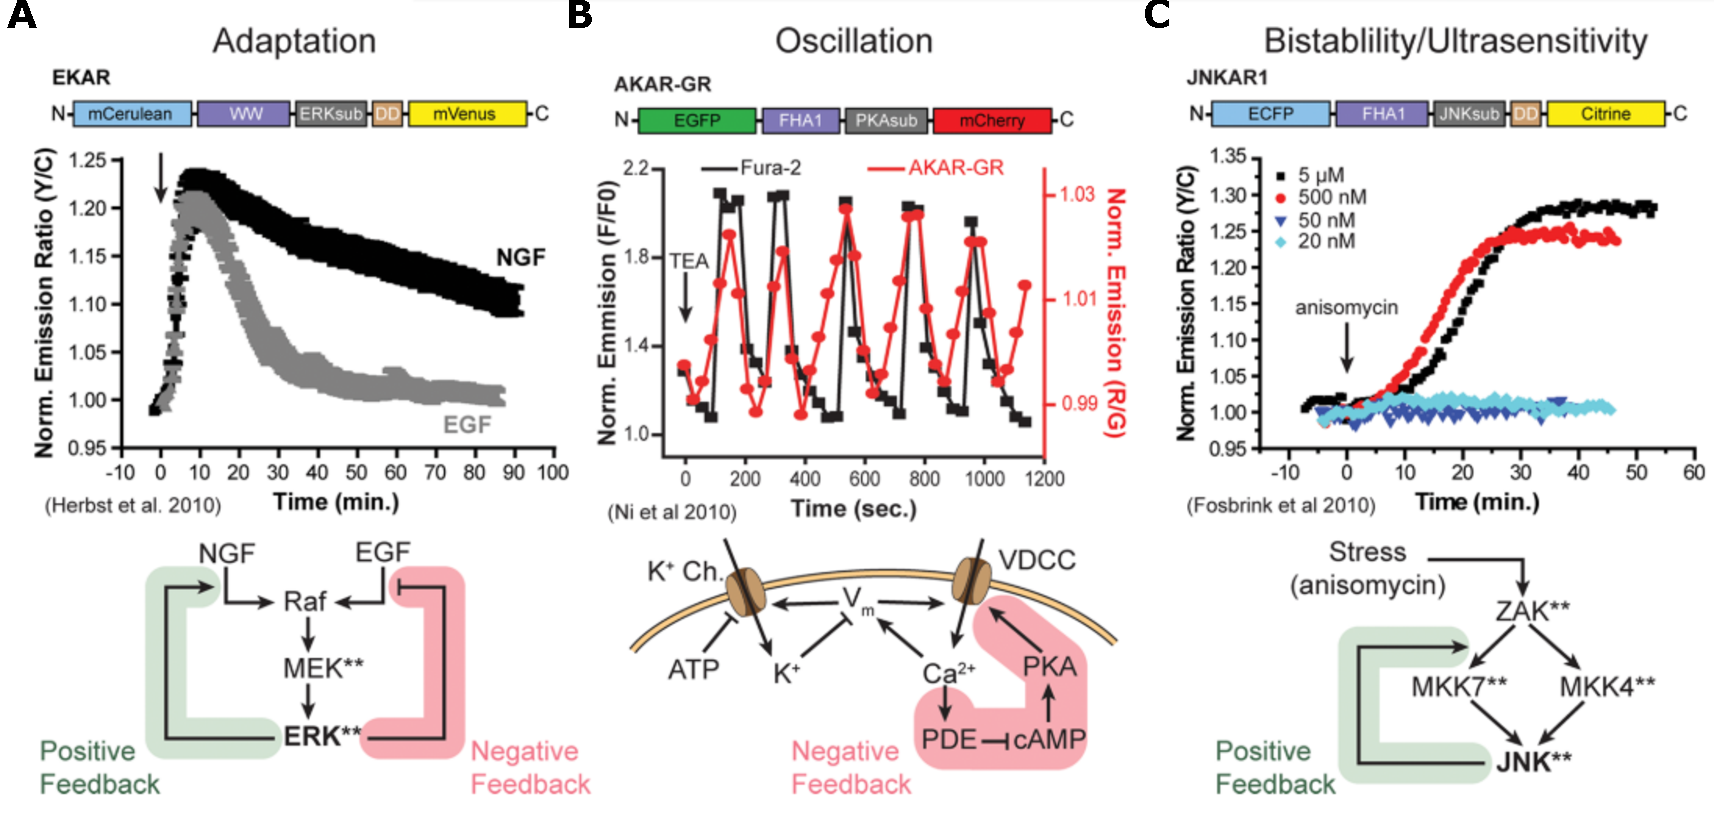
\includegraphics[width=0.9\textwidth]{img/cap_1/dinamica_temporal.pdf}
    \caption{\footnotesize{Mediciones de la dinámica temporal de distintos biosensores que ponen en evidencia comportamientos emergentes de redes biológicas. Imagen tomada de \cite{Greenwald2018}. \textbf{A.} Dinámica temporal de una respuesta adaptativa. En este caso, aunque ambos metabolitos comparten la vía de señalización, debido a diferencias en la frecuencia del estímulo, se producen respuestas distintas a nivel celular. \textbf{B.} Multiplexar la dinámica oscilatoria del Calcio intracelular permite encontrar cómo ésta se halla regulada por distintas vías. \textbf{C.} Estudiar la dinámica del reportero de actividad de JNK permite describir el comportamiento ultrasensible y biestable de la vía JNK al estrés.}}
    \label{fig:dinamica_temporal}
\end{figure}

Visualizar la dinámica mediante biosensores no solo resulta beneficioso para ver la temporalidad, sino también la variabilidad intercelular. Las oscilaciones mencionadas previamente suelen ser asincrónicas por lo que solo es posible estudiarlas si observamos a nivel de célula única. \cite{Aoki2013} demostraron a través de EKAREV, un biosensor de ERK, que pulsos de actividad en células individuales tienen un efecto paracrino sobre las células vecinas y sirven para controlar la proliferación. Incluso cuando el proceso bajo estudio puede ser sincronizado, como es el caso del ciclo celular, la variabilidad intercelular hace que las células se desfasen entre sí, dificultando su análisis.

Dada la elevada interconectividad de las redes biológicas y considerando su variabilidad, resulta crucial poder multiplexar varios nodos, es decir, observar su actividad simultáneamente. Muchas de las técnicas son discutidas por \cite{Grecco2016}. Algunas estrategias consisten en observar biosensores diferentes expresados en células distintas y relacionarlos a través de un marcador de referencia como el llamado ``multiplexado computacional''. Por ejemplo, \cite{Machacek2009} relacionan la señal obtenida de sensores para Rac1, Cdc42 y RhoA con la protrusión celular utilizando lo que se denomina multiplexado computacional. El limitante físico en la cantidad de biosensores que pueden ser visualizados en el mismo espacio está dado por el espectro disponible. Por esta razón, biosensores con espectros reducidos como los basados en homoFRET o en aplacamiento (quenching) resultan ideales. \cite{Mehta2018b} demuestran que es posible utilizar hasta seis biosensores simultáneamente, mientras sea posible confinar algunos de ellos a ciertos compartimentos subcelulares.


%%%%%%%%%%%%%%%%%%%%%%%%%%%%%%%%%%%%%%%%
\section{La red de caspasas como modelo}
\label{sec:intro:CascadaApoptotica}


%Existen numerosos modelos en los repositorios presentados en la sección \ref{sec:intro:EstudiarRedes}. Muchos de estos fueron preparados para describir el comportamiento de alguna red en un contexto específico. Debido a la carencia teórica de como combinar modelos en uno solo conservando las propiedades previas y la dificultad de agregar datos o experimentos en un solo paquete, muchos de estos modelos describen el comportamiento de distintos módulos de redes biológicas sin poder ser combinados entre sí o extrapolados a distintas situaciones. La cascada apoptótica es un claro ejemplo de esto ya que esta compuesta por varios módulos y, considerando que puede ser iniciada por distintos tipos de estímulos, la dinámica puede depender del desencadenante.

La apoptosis es un proceso de muerte celular programada que ocurre en organismos multicelulares de forma ordenada, sin liberar el contenido intracelular al espacio intercelular, evitando así dañar a las células vecinas. Para tomar esta decisión, las células integran información sobre el entorno en el que se hallan, así cómo cuánto daño celular interno acumulado contienen. Este programa juega un rol fundamental tanto durante el desarrollo embriológico de órganos, como para el mantenimiento del número de células, entre otras cosas. Es un proceso finamente regulado que cuando se altera produce graves patologías como malformaciones o aparición de tumores, así como también enfermedades neurodegenerativas por citar algunos ejemplos \citep{Kominami2012}. Contrariamente, la necrosis es un proceso de muerte desordenado que genera una serie de reacciones locales, conduciendo a respuestas de tipo inflamatorio. Entender el mecanismo de inducción de apoptosis, sin generar elevados niveles de necrosis, es importante en la generación de tratamientos para enfermedades como el cáncer.

Desde un punto de vista evolutivo, ésta cascada está muy bien conservada y los engranajes principales de la maquinaria apoptótica son las caspasas \citep{Sakamaki2009}. Estas pertenecen a una familia de proteínas denominado cisteín-proteasas y se encargan de clivar proteínas reconociendo una secuencia específica de aminoácidos. En circunstancias normales, las caspasas se hallan expresadas constitutivamente en su forma inactiva como zymógenos o procaspasas. Para gatillar la cascada de caspasas que desencadena la apoptosis se pueden estimular dos vías diferentes, intrínseca y extrínseca, que producen dinámicas distintas en el sistema. La vía intrínseca surge de señales provenientes de adentro de la célula, como estrés celular o daño al ADN, mientras que, la vía extrínseca es desencadenada por estimulación de receptores de membrana celular llamados receptores de la muerte \citep{Kominami2012a}. Su activación se encuentra regulada en numerosos puntos, siendo necesario por lo tanto una cascada de eventos para que la célula se vea irreversiblemente determinada a la apoptosis. Es posible disecar la cascada en los módulos que la componen que son el extrínseco, encargado de transducir señales extracelulares y dar inicio al proceso, el intrínseco, que inicia la cascada en respuesta a daño celular, y el efector, en el que convergen ambos módulos iniciadores para la completa ejecución del proceso (ver \cref{fig:Sketch}).

\begin{figure}
    \centering
    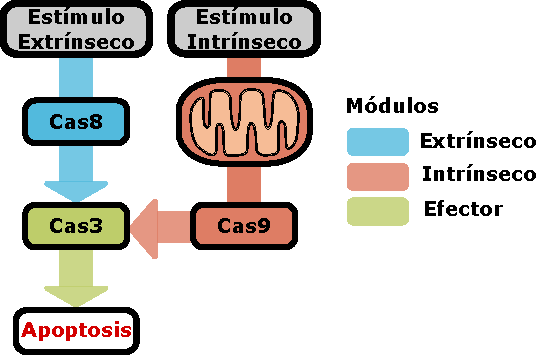
\includegraphics[width=0.5\textwidth]{img/cap_1/flujo_sketch.pdf}
    \caption{\footnotesize{Esquema del flujo de la señal en la cascada apoptótica. Ésta puede ser desencadenada por estímulos intrínsecos o extrínsecos y la señal luego converge en el módulo efector. Adaptado de \cite{Corbat2021}.}}
    \label{fig:Sketch}
\end{figure}

Los distintos módulos de la cascada apoptótica así cómo la dinámica al iniciarla a través de dos tipos de estímulo distintos fueron analizados por separado o en distintas combinaciones entre sí. Por ejemplo, \cite{Bentele2004} se concentran en analizar la respuesta de la red ante estímulos extrínsecos y cual es la sensibilidad de la dinámica ante una perturbación en cada parámetro. Por otro lado, \cite{Rehm2006} incluyen en su modelo solo los módulos intrínseco y efector y determinan la importancia de los lazos de retroalimentación en la red para superar las inhibiciones del sistema. Análogamente, \cite{Legewie2006} también analizan las vías intrínseca y efectora para recalcar la importancia de los lazos de retroalimentación positiva para generar biestabilidad en el sistema.

\begin{figure}
    \centering
    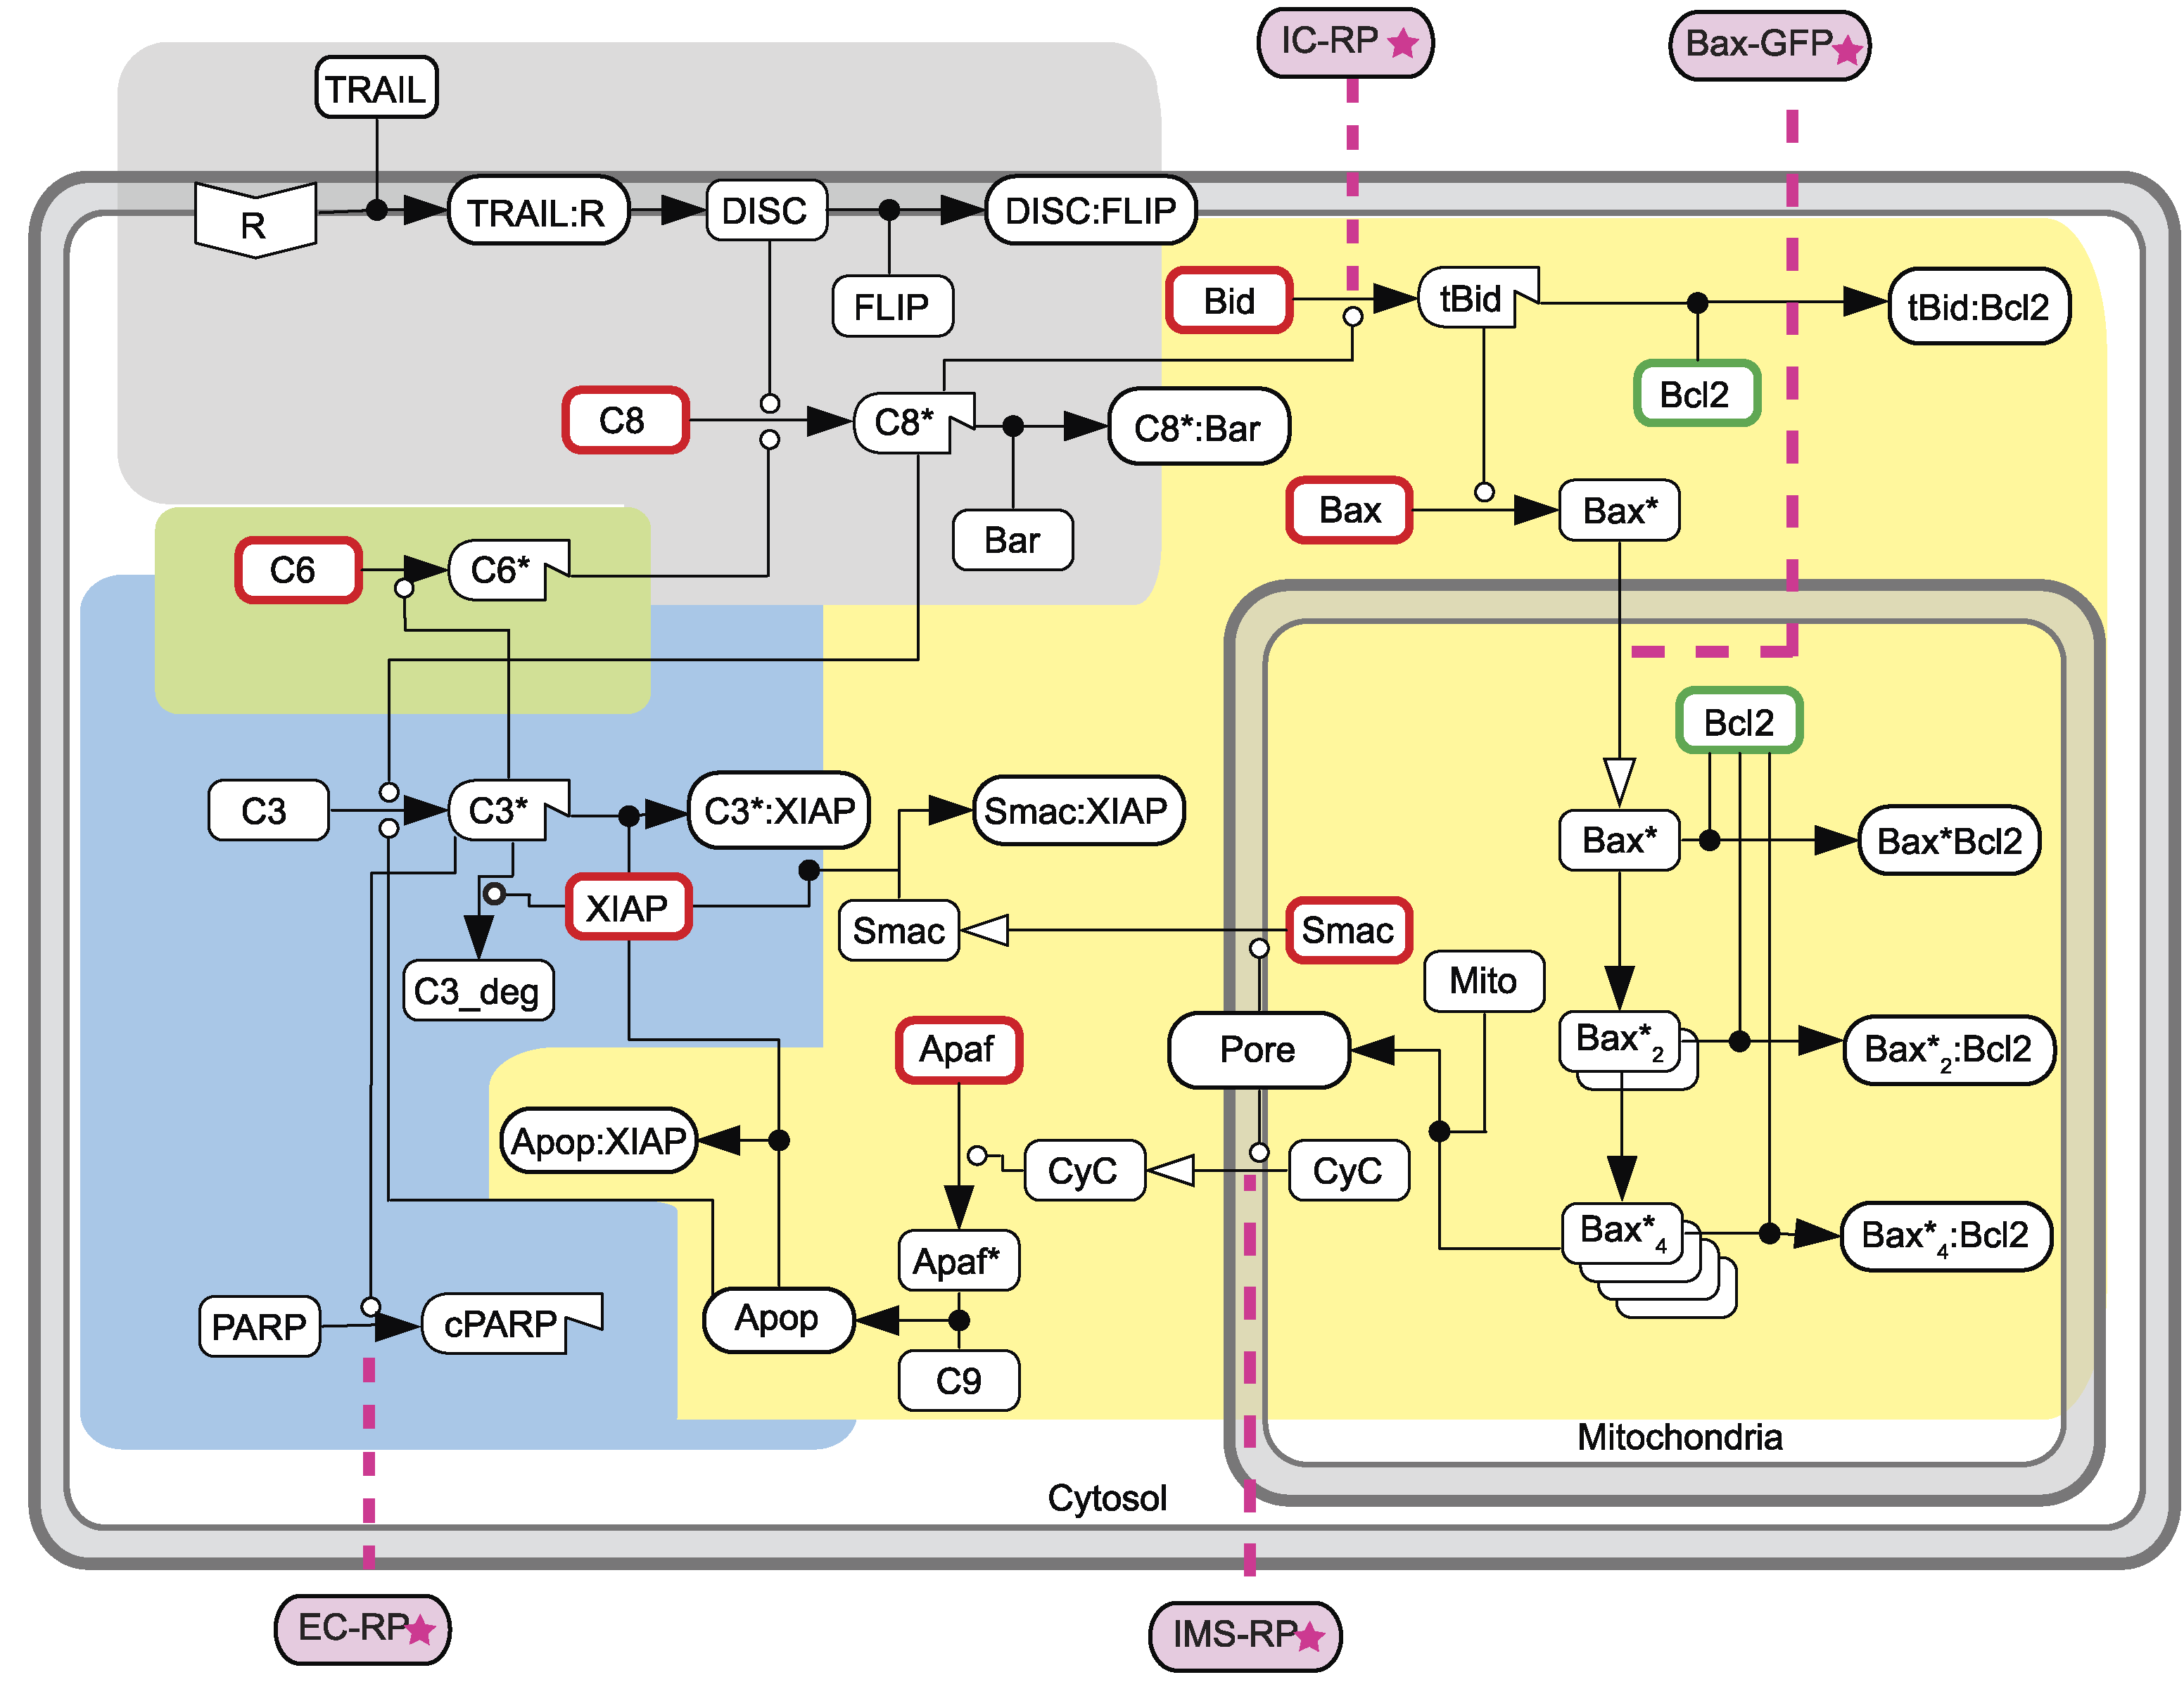
\includegraphics[width=0.8\textwidth]{img/cap_1/ModeloCompleto.png}
    \caption{\footnotesize{Esquema del modelo completo de la cascada apoptótica desarrollado por  \cite{Albeck2008}. Se pueden apreciar en colores distintos los módulos incluidos en el modelo, así como distintos compartimientos. Imagen tomada de \cite{Albeck2008}.}}
    \label{fig:ModeloCompleto}
\end{figure}

Uno de los modelos más completos de la cascada apoptótica es \ening{Extrinsic Apoptotic Reaction Model} (EARM). Éste fue desarrollado por \cite{Albeck2008} con el objetivo de describir dos características clave de la red: la variabilidad en el desencadenamiento de la cascada y la instantaneidad una vez iniciado el proceso. Para desarrollar dicho modelo, el grupo utilizó sensores basados en heteroFRET para estudiar la dinámica de la caspasa 8, iniciadora de la vía extrínseca, y la caspasa 3, efectora, en distintos experimentos perturbativos utilizando ARN de interferencia para bloquear la transducción de ciertas especies. Dicho modelo cuenta con 58 especies que corresponden a 18 moléculas cuyas condiciones iniciales son distintas de 0 y 40 especies adicionales que representan complejos, proteínas clivadas, o formas localizadas de especies iniciales que interactúan mediante 28 reacciones con 70 constantes de reacción que son no nulas (ver \cref{fig:ModeloCompleto}).

EARM se divide en cuatro módulos. El primero (gris) consiste en una representación agrupada de la unión del factor de necrosis tumoral (TNF por sus siglas en inglés) o ligando de inducción de apoptosis relacionado con TNF (TRAIL por sus siglas en inglés) al receptor y la subsecuente activación de la procaspasa 8 mediante el complejo de señalización de inducción de muerte (DISC por sus siglas en inglés) unido al receptor. En segundo lugar (azul), se muestra la cascada enzimática en que la caspasa 8 activa cliva a la procaspasa 3, la cual a su vez cliva otros sustratos efectores. Por otro lado, se muestra la vía mitocondrial (amarillo) por la cual la caspasa 8 activa trunca a Bid para dar lugar a la activación de Bax que luego dará lugar a la formación de poros en la membrana mitocondrial por los cuales citocromo C (CyC por sus siglas en inglés) y Smac son traslocados al citosol; una vez ahí, se forma el apoptosoma a partir de Apaf-1 y procaspasa 9, para clivar y activar aún más moléculas de caspasa 3. Por último, se representa (verde) un lazo de retroalimentación positivo entre la caspasa 3 y la procaspasa 8 mediado por la caspasa 6, que es clivada y activada por la caspasa 3.

Sumado a las aproximaciones implícitas en ley de acción de masas, la construcción de este modelo agrega otras tres aproximaciones que deben tenerse en cuenta. En primer lugar, la formación de DISC y el apoptosoma que incluyen unión de varias proteínas fue simplificado usando una representación con parámetros agrupados. En segundo lugar, se omitió la síntesis y degradación de cualquier proteína (exceptuando la degradación de caspasa 3 una vez unida a XIAP). Por último, especies con actividades similares fueron representadas por una única especie, entre ellas están: caspasa 8 y caspasa 10, caspasa 3 y caspasa 7 y la familia de proteínas similares a Bcl-2.

Por otro lado, \cite{Zhang2009} hacen un análisis modular de la cascada apoptótica intrínsecamente estimulada. En su trabajo, dividen la cascada en: un módulo iniciador que integra señales provenientes del sensado de daño genético (relacionado principalmente con p53) que culmina con la activación BAX; un módulo amplificador que inicia con BAX formando poros en la membrana mitocondrial y rápidamente liberando el contenido mitocondrial al citoplasma; y el módulo ejecutor que incluye la formación y activación del apoptosoma y la caspasa intrínseca, así como la caspasa efectora. Cabe destacar que la rápida liberación del contenido mitocondrial se condice con los resultados observados y descriptos por \cite{Albeck2008}.

Entre los biosensores basados en FRET se encuentra un grupo capaz de sensar actividad de proteasas. Estos consisten en dos fluoróforos unidos por una secuencia sensible a la actividad de la proteasa en estudio. Las propiedades espectroscópicas de los fluoróforos seleccionados son tales que, cuando el biosensor se halla en estado dimérico, ocurra una transferencia de energía por resonancia de Förster entre ellos. Así, cuantificando dicha transferencia de energía, es posible estimar la proporción de biosensores en estado dimérico o monomérico \citep{Greenwald2018}. En los trabajos de \cite{Tyas2000} y \cite{Rehm2002} utilizan fluoróforos cyan y amarillos unidos por la secuencia DEVD, reconocida por la caspasa efectora, para mostrar que la actividad de la caspasa ocurre rápidamente en un intervalo de tiempo reducido (del orden de 15 minutos), mientras que el instante en el que ocurre es mucho más variable (del orden de horas) y depende de otros factores como tipo celular, droga y concentración usadas, entre otros. Dentro del grupo, \cite{Stegemann2015} utilizan un biosensor basado en homoFRET que consiste en dos fluoróforos de mCitrine unidos por la secuencia DEVD y cuyo estado puede analizarse mediante microscopía de anisotropía en polarización. En el trabajo analizan la dinámica de apoptosis al utilizar substratos fotoinducibles, disueltos o fijos en superficies, que generan especies reactivas del oxígeno. Cabe destacar que, aunque el sustrato disuelto genera elevados niveles de muerte celular, cuando se encuentra fijo a una superficie, actúa como factor protector (ver \cref{fig:stegemann}).

\begin{figure}
    \centering
    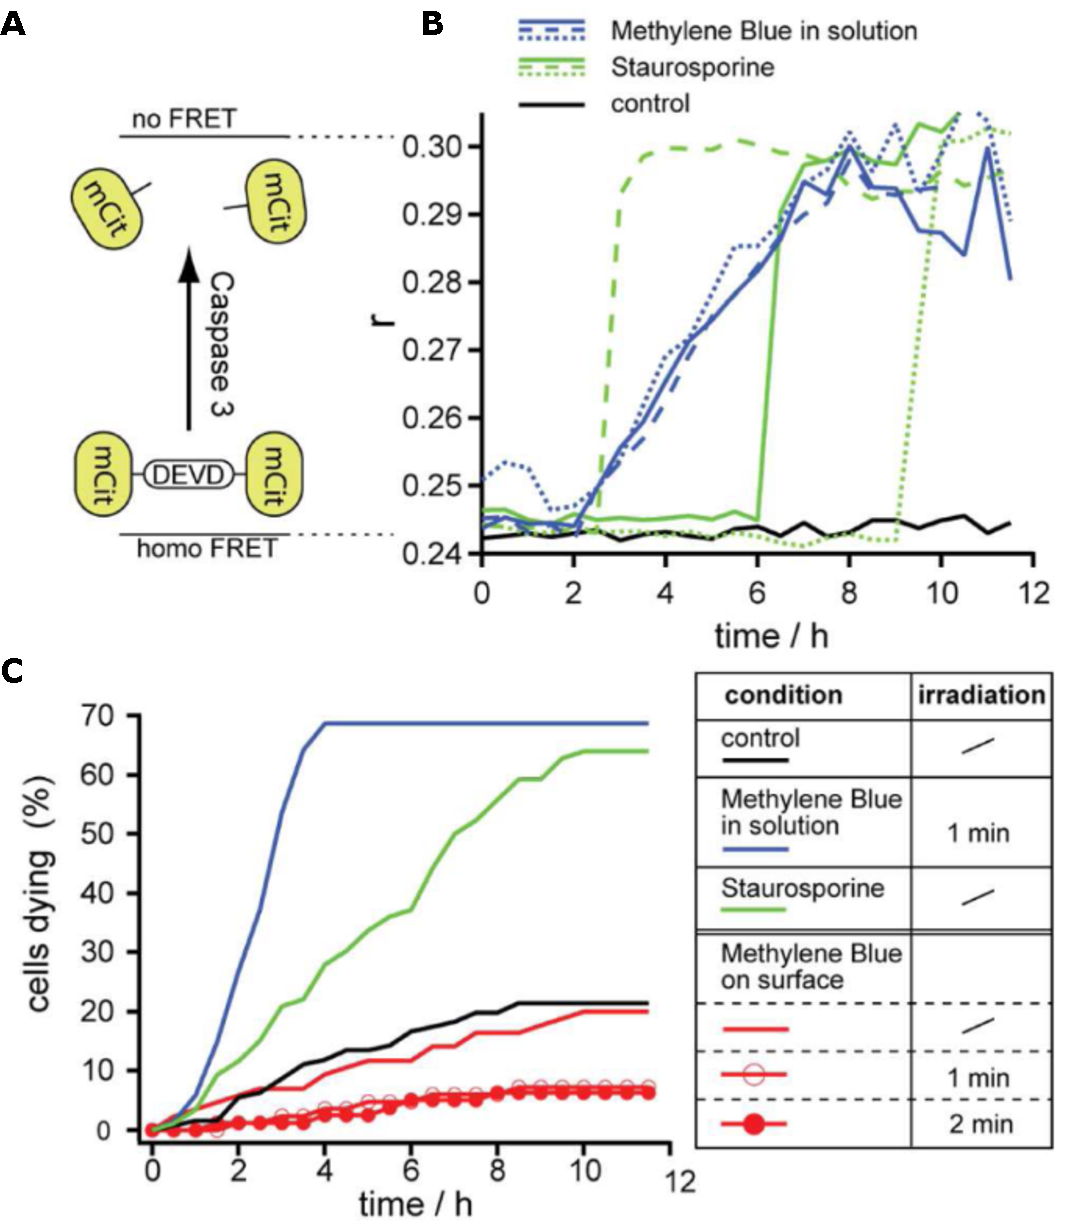
\includegraphics[width=0.6\textwidth]{img/cap_1/stegemann.pdf}
    \caption{\footnotesize{\textbf{A.} Descripción esquemática del biosensor de caspasa 3 basado en homoFRET. \textbf{B.} Curvas de anisotropía correspondientes al biosensor de caspasa 3 transfectado en células que fueron sujetas a tratamientos con staurosporina o azul de metileno. \textbf{C.} Porcentaje de células que sobreviven ante tratamientos con staurosporina o azul de metileno en solución o las superficies funcionalizadas con azul de metileno y luego fotoinducidas. Es interesante notar que las células expuestas a azul de metileno disuelto e irradiadas muestran un elevado porcentaje de muerte celular mientras que las que fueron expuestas a superficies funcionalizadas con azul de metileno e irradiadas muestran menor muerte celular que el caso control.  Imagen tomada de \cite{Stegemann2015}.}}
    \label{fig:stegemann}
\end{figure}

En conclusión, la red de caspasas es ideal para poner a punto diversas metodologías para estudiar y simular redes biológicas. Cada uno de los módulos de la cascada apoptótica tiene una caspasa cuya actividad de proteasa puede ser observada a través de biosensores análogos a los previamente descriptos. Además, la cantidad de estos módulos es suficiente como para poder multiplexarlos a nivel de célula única por medio de biosensores basados en homoFRET. Por último, la extensa librería de modelos describiendo partes o la totalidad de la red brinda un buen punto de partida y los variados experimentos caracterizando distintos comportamientos de la red dan cuenta de los comportamientos que deben emerger del modelo.


%%%%%%%%%%%%%%%%%%%%%%%%%%%%%%%%%%%%%%%%
\section{Esquema de la Tesis}

El objetivo de este trabajo fue generar un modelo matemático para describir la dinámica de la red de caspasas en distintos contextos biológicos. Tener una visión más integrada de la red será útil para comprender mejor la interconectividad entre sus módulos así como para plantear diversas soluciones terapéuticas. Además, el flujo de trabajo utilizado podría ser aplicado para el estudio de otros sistemas en dónde también se integre información.

% Para ello fue necesario confeccionar un paquete de datos que amalgame experimentos realizados en contextos distintos y cuyos observables pueden ser fácilmente comparados con predicciones del modelo. Considerando éste objetivo específico, fue necesario desarrollar e implementar un biosensor capaz de interrogar varios nodos de la red, simultáneamente y a nivel de célula única y minimizar la perturbación introducida. 

En primer lugar, en el capítulo 2 presentaré cómo realizar y analizar experimentos utilizando un sensor genérico análogo al presentado en el trabajo de \cite{Stegemann2015}. Para ello describiré un modelo mínimo utilizando uno de estos sensores, en qué consiste la microscopía de anisotropía en polarización y como analizar las imágenes obtenidas para obtener un observable robusto y comparable entre experimentos y con los resultados del modelado. El análisis desarrollado se encuentra publicado en \cite{Corbat2018}.

Luego, en el capítulo 3 describiré los biosensores basados en homoFRET utilizados para los distintos experimentos. Discutiré cómo fueron seleccionados los pares de fluoróforos, el diseño de los plásmidos utilizados y la metodología utilizada para reducir las perturbaciones que introducen en el sistema. El estudio de los distintos pares de fluoróforos se encuentra presentado en \cite{Corbat2018}, mientras que las mejoras introducidas al biosensor y el efecto de sus perturbaciones en la red se haya publicado en \cite{Habif2021}.

Finalmente, en el capítulo 4 analizaremos los resultados de distintos experimentos donde se indague la dinámica de la red apoptótica para generar un modelo integrador de todos los módulos de la red. Una vez generado dicho modelo, mostraré su capacidad predictiva ante distintos experimentos realizados previamente y así verificar que no se redujo su capacidad predictiva. Un primer modelo describiendo el comportamiento de la red ante estímulos extrínsecos se haya presentado en \cite{Corbat2018}, mientras que el modelo integrador que describe el comportamiento de la cascada ante distintos estímulos y en contextos diferentes se encuentra en \cite{Corbat2021}.